\documentclass[../main.tex]{subfiles}

\begin{document}

\section{Brainhack Cloud}

\authors{Steffen Bollmann\textsuperscript{1,2}, Isil Bilgin\textsuperscript{3}, Peer Herholz\textsuperscript{4}, Rémi Gau\textsuperscript{5}, Samuel Guay\textsuperscript{6}, Johanna Bayer\textsuperscript{7,8}}

\affiliations{1. School of Information Technology and Electrical Engineering, The University of Queensland, Brisbane, Australia, 2. Centre for Innovation in Biomedical Imaging Technology, University of Queensland, Brisbane, Australia, 3. Centre de recherche de l'Institut universitaire de gériatrie de Montréal, University of Montreal, Canada, 4. NeuroDataSciene - ORIGAMI lab, Montreal Neurological Institute-Hospital, McGill University, 5. Institut de recherche en sciences psychologique, Université catholique de Louvain. Louvain la neuve, Belgique, 6. Department of Psychology, University of Montreal, Canada, 7. Centre for Youth Mental Health, the University of Melbourne, Australia, 8. Orygen Youth Health, Australia.}

Today’s neuroscientific research deals with vast amounts of electrophysiological, neuroimaging and behavioural data. The progress in the field is enabled by the widespread availability of powerful computing and storage resources. Cloud computing in particular offers the opportunity to flexibly scale resources and it enables global collaboration across institutions. However, cloud computing is currently not widely used in the neuroscience field, although it could provide important scientific, economical, and environmental gains considering its effect in collaboration and sustainability \parencite{apon2015, OracleSustainabilty}. One problem is the availability of cloud resources for researchers, because Universities commonly only provide on-premise high performance computing resources. The second problem is that many researchers lack the knowledge on how to efficiently use cloud resources. This project aims to address both problems by providing free access to cloud resources for the brain imaging community and by providing targeted training and support.

A team of brainhack volunteers (https://brainhack.org/brainhack\_cloud/admins/team/) applied for Oracle Cloud Credits to support open-source projects in and around brainhack with cloud resources. The project was generously funded by Oracle Cloud for Research \parencite{OracleResearch} with \$230,000.00 AUD from the 29th of January 2022 until the 28th of January 2024. To facilitate the uptake of cloud computing in the field, the team built several resources (https://brainhack.org/brainhack\_cloud/tutorials/) to lower the entry barriers for members of the Brainhack community. 

During the 2022 Brainhack, the team gave a presentation to share the capabilities that cloud computing offers to the Brainhack community, how they can place their resource requests and where they can get help. In total 11 projects were onboarded to the cloud and supported in their specific use cases: One team utilised the latest GPU architecture to take part in the Anatomical Tracings of Lesions After Stroke Grand Challenge. Others developed continuous integration tests for their tools using for example a full Slurm HPC cluster in the cloud to test how their tool behaves in such an environment. Another group deployed the Neurodesk.org \parencite{NeuroDesk} project on a Kubernetes cluster to make it available for a student cohort to learn about neuroimage processing and to get access to all neuroimaging tools via the browser. All projects will have access to these cloud resources until 2024 and we are continuously onboarding new projects onto the cloud (https://brainhack.org/brainhack\_cloud/docs/request/).

The Brainhack Cloud team plans to run a series of training modules in various Brainhack events throughout the year to reach researchers from various backgrounds and increase their familiarity with the resources provided for the community while providing free and fair access to the computational resources. The training modules will cover how to use and access computing and storage resources (e.g., generating SSH keys), to more advanced levels covering the use of cloud native technology like software containers (e.g., Docker/Singularity), container orchestration (e.g., Kubernetes), object storage (e.g, S3), and infrastructure as code (e.g., Terraform).

\begin{figure}
    \centering
    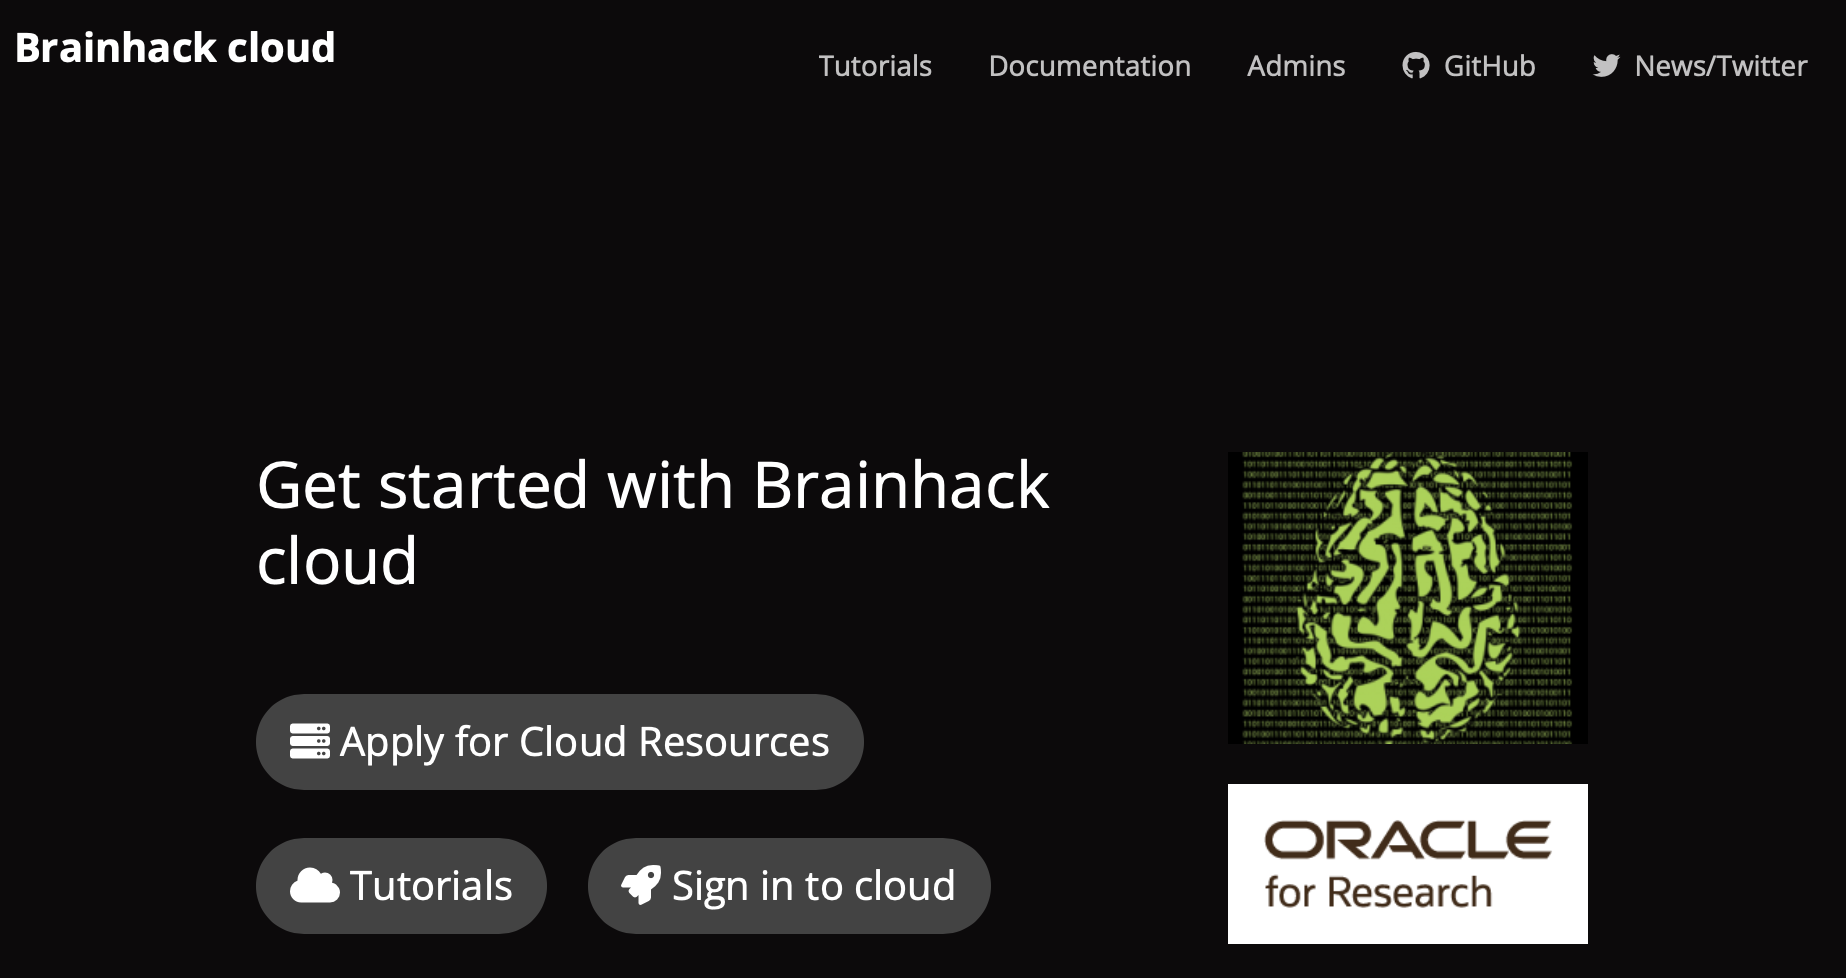
\includegraphics[width=0.5\textwidth]{brainhack_cloud.png}
    \caption{A team of brainhack volunteers, applied for Oracle Cloud Credits to support open source projects in and around brainhack with powerful cloud resources on the Oracle Cloud: https://brainhack.org/brainhack\_cloud/
    }
    \label{fig:cloud}
\end{figure}


% References|
%     1. Apon, A. W., Ngo, L. B., Payne, M. E., \& Wilson, P. W. (2015). Assessing the effect of high performance computing capabilities on academic research output. Empirical Economics, 48(1), 283-312.
%     2. Oracle cloud sustainability, https://www.oracle.com/uk/sustainability/green-cloud/
%     3. Oracle for Research, https://docs.oracle.com/en/programs/research/
%     4. NeuroDesk, https://www.neurodesk.org/


\printbibliography


\end{document}
